\documentclass[a4paper, 12pt]{scrartcl}

\usepackage{a4wide}
\usepackage[utf8]{inputenc}
\usepackage[ngerman]{babel}
\usepackage[T1]{fontenc}
\usepackage{amsmath}
\usepackage{graphicx}
\usepackage{listings}
\usepackage{hyperref}

\usepackage{tikz}
\usetikzlibrary{positioning,calc,shapes,arrows,shapes.multipart}

\usepackage{scrpage2}
\pagestyle{scrheadings}
\clearscrheadfoot

\makeatletter

\def \autoren {Felix Starke, Lars Hübner}
\def \titel {Metronom für Intel 8051}
\def \arbeit {Projekt Systemnahe Programmierung}
\def \uni {DHBW Karlsruhe}
\def \betreuer {Herr Lausen}
\def \datum {6. Juni 2018}

\title{\titel}
\author{\autoren}
\date{\datum}

\ihead{\titel}
\ohead{\autoren}
\ofoot{\pagemark}

\begin{document}

\begin{titlepage}
	\centering
	
\includegraphics[width=0.4\textwidth]{dhbw.png}\par\vspace{1cm}
	{\scshape\LARGE \uni \par}
	\vspace{1cm}
	{\scshape\Large \arbeit\par}
	\vspace{1.5cm}
	{\huge\bfseries \titel\par}
	\vspace{2cm}
	{\Large\itshape \autoren\par}
	\vfill
	betreut von\par
	\textsc{\betreuer}

	\vfill

% Bottom of the page
	{\large \datum\par}
\end{titlepage}

\newpage
\tableofcontents
\newpage

\section{Einleitung}
\subsection{Motivation}

Ein Metronom beschreibt ein mechanisches oder elektronisches Gerät, welches zur regelmäßigen Tonerzeugung genutzt wird um musikalische Rhythmen zu unterstützen. Die Mehrzahl der neueren Metronome haben eine Funktion, bei der über ein regelmäßiges Klicken auf einen Button der entsprechende Klick-Takt übernommen wird.
\\
Da Metronome häufig als kleine portable Geräte mit geringem Stromverbrauch umgesetzt werden, kann eine entsprechende Funktionalität auf einem Intel 8051 Mikrocontroller implementiert werden. Die Programmierung auf diesem Mikrocomputer geschieht in Assembler. Ziel dieses Projektes ist entsprechend die Implementierung einer solchen "Tap to Beat" Funktion in Assembler für den 8051.

\subsection{Aufgabenstellung}
Aus diesen Anforderungen ergibt sich die folgende Aufgabenstellung.
\\
Das Programm muss eine Funktionalität implementieren, die das Aufnehmen des Taktes über eine Eingabehardware ermöglicht. Außerdem muss das Ausgeben des Taktes über eine passende Ausgabehardware implementiert werden.
Das gesamte Programm lässt sich damit in zwei große Teile splitten, dass Recording und das Anzeigen des Taktes.
\\
\\
\textbf{Recording}
\\
Die Aufnahme des Taktes muss über eine Eingabehardware getätigt werden. In diesem Projekt wurde eine Keypad-Matrix mit Tasten als Eingabe gewählt. Über eine dieser Tasten soll nun der Takt gemessen werden. Hierzu wird jeweils die Zeitspanne zwischen zwei Tastendrücken mithilfe eines Timers gemessen. Die Messungen sollen im Anschluss auf summiert und am Ende durch die Anzahl der Messungen geteilt werden, um den Mittelwert zu erhalten.
\\
\\
\textbf{Display Metronom}
\\
Nachdem der durchschnittliche Takt gemessen und ermittelt wurde, gilt es diesen auf einem Ausgabemedium anzuzeigen. Anstelle einer Tonausgabe wird in dieser Implementierung eine LED-Matrix genutzt um den Takt zu visualisieren.
\newpage
\section{Grundlagen}
\subsection{Assembler}
\subsection{Intel 8051 Mikrocontroller}
\subsection{Entwicklungsumgebung MCU-8051}

\newpage
\section{Konzept}
\subsection{Eingaben, Ausgaben und Ports}
Um dem Metronom den Takt vorzugeben, kommt eine 4x4 Keypad-Matrix (siehe \autoref{fig:keypad}) zur Eingabe zum Einsatz. Diese ist an alle acht Pins von Port 0 angeschlossen. Dabei werden die Pins 0-3 für die vier Spalten der Matrix und Pins 4-7 für die Zeilen der Matrix verwendet. Um eine gedrückte Teste zu detektieren müssen zunächst die Pins 0-3 auf "1" gesetzt werden und die Pins 4-7 gelesen werden. So lässt sich herausfinden, ob überhaupt eine Taste gedrückt ist und welcher Spalte diese angehört. Im nächsten Takt können dann die Pins 4-7 auf "1" gesetzt werden und 0-3 auf "0". Anschließend kann die Zeile der gedrückten Taste ermittelt werden.
\begin{figure}[h]
\centering
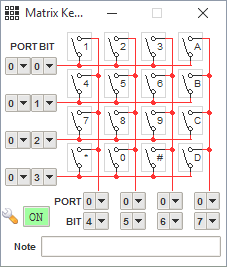
\includegraphics[width=0.5\textwidth]{keypad.png}
\caption{Keypad Matrix}
\label{fig:keypad}
\end{figure}
\\
\\
Für die Ausgabe des ermittelten Taktes wird eine 8x8 LED-Matrix (siehe \autoref{fig:led}) verwendet. diese ist an die Ports 2 und 3 angeschlossen. Die acht Pins von Port 2 werden genutzt um die Spalten der Matrix anzusteuern, die acht Pins von Port 3 werden für die Zeilen der LED-Matrix verwendet. Eine der 64 LED's leuchtet genau dann, wenn sowohl der Pin der entsprechenden Zeile als auch der entsprechenden Spalte gesetzt sind.
\begin{figure}[h]
\centering
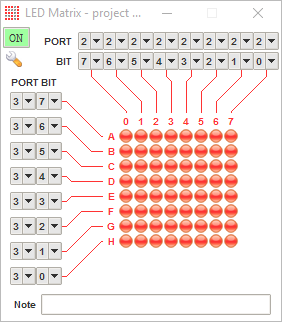
\includegraphics[width=0.5\textwidth]{led.png}
\caption{LED Matrix}
\label{fig:led}
\end{figure}
\subsection{Programmablauf}

% Include flow chart definition
% Define block styles
\tikzset{
   papDecision/.style = {
         diamond,
         draw, 
         text width = 20 mm, 
         align = center, 
         text badly centered,
         inner sep = 1 pt,
         font=\ttfamily\footnotesize,
         %line width = 1,
         minimum width = 30mm,
         minimum height = 7mm,
      },
   papStart/.style = {
         rectangle,
         draw, 
         align = center, 
         text width = 3cm, 
         text badly centered,
         inner sep = 4 pt,
         rounded corners=10pt,
         font=\ttfamily\footnotesize,
         %line width = 1,
         minimum width = 30mm,
         minimum height = 7mm,
      },
   papEnd/.style = {
         rectangle,
         draw, 
         align = center, 
         text width = 3cm, 
         text badly centered,
         inner sep = 4 pt,
         rounded corners=10pt,
         font=\ttfamily\footnotesize,
         %line width = 1,
         minimum width = 30mm,
         minimum height = 7mm,
      },
   papData/.style = {
         trapezium,
         draw, 
         align = center, 
         text width = 20 mm, 
         text badly centered,
         inner sep = 4 pt,
         trapezium left angle=70,
         trapezium right angle=110,
         font=\ttfamily\footnotesize,
         %line width = 1,
         minimum width = 30mm,
         minimum height = 7mm,
      },
   papPredProc/.style = {
         draw,
         rectangle split,
         rectangle split horizontal,
         rectangle split parts = 3,
         rectangle split empty part width=-8pt,
         align = center, 
 %       text width = 4.5 em, 
         text badly centered,
 %        inner sep = 4 pt,
         font=\ttfamily\footnotesize,
         %line width = 1,
         minimum width = 30mm,
         minimum height = 7mm,
      },
   papProcess/.style = {
         rectangle,
         draw,
         align = center, 
         text width = 3cm, 
         text badly centered,
         %inner sep = 2 pt,
         font=\ttfamily\footnotesize,
         %line width = 1,
         minimum width = 30mm,
         minimum height = 7mm,
      },
   papLine/.style = {
         draw,
         -stealth,
         font=\ttfamily\footnotesize,
         %line width = 1,
      },
}

\newcommand{\papYes}{ja}
\newcommand{\papNo}{nein}


%%%%%%%%%%%%%%%%%%%%%%%%%%%%%%%%%%%%%%%%%%%%%%%%%%%%%%%%%%%%%%%%%


\begin{figure}
\centering
\begin{tikzpicture}[node distance = 2cm, auto]

% Place nodes
\node [papStart] (Start1){Start};
\node [papProcess, below of = Start1] (pro1){Warte auf button};
\node [papDecision, below of = pro1, yshift= -9mm](dec1){Button gedrückt?};
\node [papProcess, below of = dec1] (pro2){Starte Timer};
\node [papProcess, below of = pro2] (pro3){Warte auf button};
\node [papDecision, below of = pro3, yshift= -9mm](dec2){Button losgelassen?};
\node [papProcess, below of = dec2] (pro4){Stope Timer};
\node [papProcess, below of = pro4] (pro5){Summiere Timer auf};
\node [papDecision, below of = pro5, yshift= -9mm](dec3){Button 3x gedrückt?};
\node [papProcess, below of = dec3] (pro6){Dividiere Summe durch 3};
\node [papEnd, below of = pro6] (End) {Starte Metronom};


% Draw edges
\path [papLine] (Start1) -- (pro1);
\path [papLine] (pro1) -- (dec1);
\path [papLine] (dec1.east) -| node [right] {\papNo}(2, -2) -- (pro1.east);
\path [papLine] (dec1) -- node [right] {\papYes} (pro2);
\path [papLine] (pro2) -- (pro3);
\path [papLine] (pro3) -- (dec2);
\path [papLine] (dec2.east) -| node [right] {\papNo}(2, -8.9) -- (pro3.east);
\path [papLine] (dec2) -- node [right] {\papYes} (pro4);
\path [papLine] (pro4) -- (pro5);
\path [papLine] (pro5) -- (dec3);
\path [papLine] (dec3.east) -| node [right] {\papNo}(4, -2) -- (pro1.east);
\path [papLine] (dec3) -- node [right] {\papYes} (pro6);
\path [papLine] (pro6) -- (End);

\end{tikzpicture}
\caption{Programmablauf} \label{fig:pgmAblauf}
\end{figure}

\section{Besondere Schwierigkeiten}
Besondere Schwierigkeiten ergaben sich aufgrund der hohen Laufzeiten durch die Entwicklungsumgebung. Vorallem die Nutzung virtueller Hardware verlangsamt den Ablauf des Programms stark. So vergehen, auf einem recht leistungsstarken Rechner, etwa 7 Sekunden, bis im Simulator der Entwicklungsumgebung eine Millisekunde verstrichen ist. Da gutes Timing für ein Metronom sehr wichtig ist, musste entschieden werden, wie mit der langsamen Laufzeit umgegangen werden sollte. Da das Metronom nutzbar sein sollte wurde das Timing nicht an der simulierten Laufzeit der Entwicklungsumgebung orientiert. Da weder die Eingabe zur Festlegung des Taktes noch die Ausgabe des Takts über die LED-Matrix an die Zeit der Simulation gebunden sind, ist es einfach möglich, beides zu synchronisieren und so umzusetzten, dass das Metronom nutzbar ist.
\\

\section{Zusammenfassung}

\section{Literatur}
\section{Eidesstattliche Versicherung}
\end{document}
